\documentclass[final]{beamer}
% http://tex.stackexchange.com/questions/56205/wrapfigure-beamer-style
\usepackage{color}
%\usepackage{cutwin}
%\usetheme{RJH}
\usetheme{Berkeley}
%\usetheme{Bergen}
\usepackage[orientation=portrait,size=a0,scale=1.4,debug]{beamerposter}
\usepackage[absolute,overlay]{textpos}
\setlength{\TPHorizModule}{1cm}
\setlength{\TPVertModule}{1cm}
\beamertemplatenavigationsymbolsempty
% RGB (145,201,219), #91C9DB
%\definecolor{mybluelabel}{RGB}{145,201,219}
% RGB (48,174,228), #30AEE4
\definecolor{mybluelabel}{RGB}{48,174,228}

\begin{document}
\begin{frame}{} 

\begin{textblock}{20}(2,2)
\begin{center}
\begin{figure}[tbph]
\centering
%\includegraphics[width=0.45\textwidth]{dianahep-logo.png}

\includegraphics[width=0.70\textwidth]{images/diana-hep-06-logo-horizontal.png}
\end{figure}
\url{http://s2i2-hep.org}
\end{center}
\end{textblock}


\begin{textblock}{84.0}(6,2)
\usebackgroundtemplate{
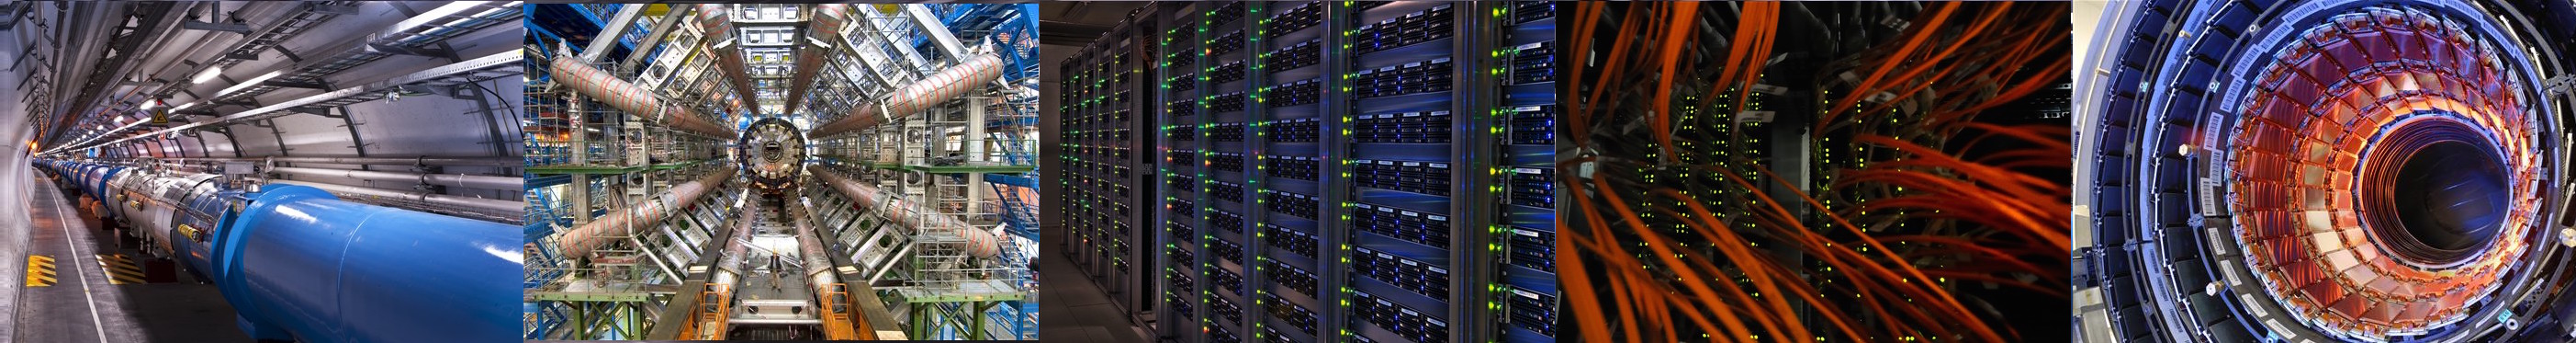
\includegraphics[width=\paperwidth,
height=\paperheight]{images/s2i2-banner.jpg}
}
\begin{center}
\begin{LARGE}
S2I2-HEP - Conceptualization of an S2I2 Institute for High Energy Physics
\end{LARGE}
\end{center}
\end{textblock}

\begin{textblock}{84.0}(6,5)
\begin{center}
\begin{Large}
PIs: Peter Elmer (Princeton U.), Mark Neubauer (U.Illinois Urbana-Champaign), \\ Mike Sokoloff (U.Cincinnati)
\end{Large}
\end{center}
\end{textblock}

\begin{textblock}{38.0}(4,10)
\begin{block}{High Energy Physics (HEP)}
%\begin{center}
The quest to understand the fundamental building blocks of nature,
and their interactions, is one of the longest running and most
ambitious of human endeavors. Facilities such as the Large Hadron
Collider (LHC), where we do our research, represent a huge step
forward in our ability to answer these questions. The discovery of
the Higgs boson, the observation of exceedingly rare decays of B
mesons, and exclusion of countless theories beyond the Standard
Model (SM) of particle physics demonstrate that these experiments
deliver results. However, the most interesting fundamental physics
questions remain wide open, amongst them: What is the dark matter
which pervades the universe? Does space-time have additional
symmetries or extend beyond the 3 spatial dimensions we know? What
is the mechanism stabilizing the Higgs mass from enormous quantum
corrections? Are neutrinos, whose only SM interactions are weak,
their own anti-particles? Can the theories of gravity and quantum
mechanics be reconciled? Planned and running HEP experiments 
aim to answer these questions over the next 20 years.
~~~ \\
~~~ \\
\begin{figure}[tbph]
\centering
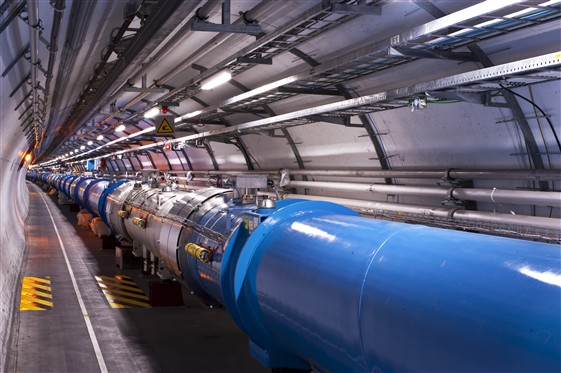
\includegraphics[width=0.48\textwidth]{images/0910152_02-A5-at-72-dpi.jpg}
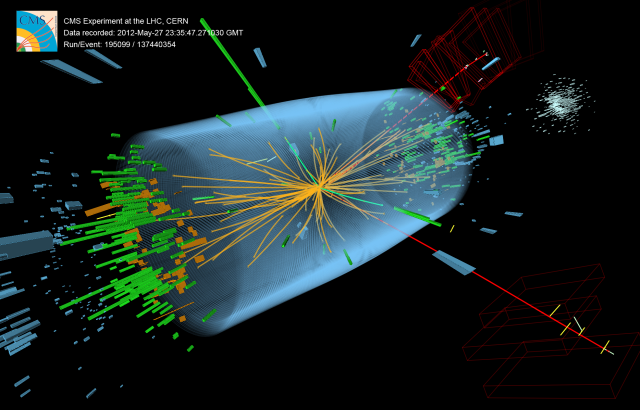
\includegraphics[width=0.50\textwidth]{images/eemm_run195099_evt137440354_ispy_3d-annotated-2.png}
\begin{center}
{\small \copyright~2009-2016 CERN (License: CC-BY-SA-4.0)}
\end{center}
\end{figure}
\end{block}
\end{textblock}




%\begin{textblock}{38.0}(4,10)
\begin{textblock}{38.0}(44,10)
\begin{block}{The DIANA/HEP Project}
The primary goal of DIANA/HEP is to develop state-of-the-art tools
for experiments which acquire, reduce, and analyze petabytes of
data. Improving performance, interoperability, and collaborative
tools through modifications and additions to ROOT and other packages
broadly used by the community will allow users to more fully exploit
the data being acquired at CERN's Large Hadron Collider (LHC) and
other facilities. The LHC experiments, for example, use nearly 0.5 Exabyte of
storage today, and planned upgrades through the 2020s will increase this
by more than a factor of 100. 
%\begin{figure}[tbph]
%\centering
%\includegraphics[width=0.8\textwidth]{diana-hep-goals.png}
%\end{figure}
\end{block}
\end{textblock}






\begin{textblock}{38.0}(44,25.0)
\begin{block}{The HEP Analysis Software Ecosystem}
ROOT (\url{https://root.cern.ch}) is
the {\em de-facto} home for most community analysis
software developed in particle physics and related fields. Begun at CERN in 1995,
it provides a sophisticated data format and serialization technology
%(used, as an example, for 200 PB of LHC Run 1 data)
as well as key software tools for
data modeling, likelihood fitting, statistics and
multivariate data analysis. It also has a broader range of
functionalities, not strictly tied to the data-intensive aspects
of our science, including interactive C++ analysis, histogramming,
graphics (2D and 3D), math libraries (matrix algebra), image manipulation,
and tools for distributed computing. Despite many pioneering and
innovative features, the components are seen as too coupled,
and limited by design decisions taken 20 years ago.
Given the challenges from technology evolution and analysis complexity,
we are at a point in the software lifecycle where large changes are needed,
much as ROOT replaced an earlier generation of
FORTRAN-based tools (PAW, HBOOK).
%ROOT is, however, the starting
%point for any plan to enable the our community to
%exploit exabyte-scale data sets.
DIANA/HEP is building on and improving these
community libraries, moving other existing software elements into
community libraries, and developing additional new tools.
\end{block}
\end{textblock}







\begin{textblock}{38.0}(44,102)
\begin{block}{Acknowledgement}
This project is supported by National Science Foundation grants ACI-1558216, ACI-1558219, and ACI-1558233. Any opinions, findings, conclusions or recommendations expressed in this material are those of the developers and do not necessarily reflect the views of the National Science Foundation.
\end{block}
\end{textblock}




\end{frame}
\end{document}
